%%%%%%%%%%%%%%%%%%%%%%%%%%%%%%%%%%%%%%%%%%%%%%%%%%%%%%%%%%%%%%%%%%%%%%
% LaTeX Example: Project Report
%
% Source: http://www.howtotex.com
%
% Feel free to distribute this example, but please keep the referral
% to howtotex.com
% Date: March 2011 
% 
%%%%%%%%%%%%%%%%%%%%%%%%%%%%%%%%%%%%%%%%%%%%%%%%%%%%%%%%%%%%%%%%%%%%%%
% How to use writeLaTeX: 
%
% You edit the source code here on the left, and the preview on the
% right shows you the result within a few seconds.
%
% Bookmark this page and share the URL with your co-authors. They can
% edit at the same time!
%
% You can upload figures, bibliographies, custom classes and
% styles using the files menu.
%
% If you're new to LaTeX, the wikibook is a great place to start:
% http://en.wikibooks.org/wiki/LaTeX
%
%%%%%%%%%%%%%%%%%%%%%%%%%%%%%%%%%%%%%%%%%%%%%%%%%%%%%%%%%%%%%%%%%%%%%%
% Edit the title below to update the display in My Documents
%\title{Project Report}
%
%%% Preamble
\documentclass[paper=a4, fontsize=11pt]{scrartcl}
\usepackage[T1]{fontenc}
\usepackage{fourier}

\usepackage[english]{babel}															% English language/hyphenation
\usepackage[protrusion=true,expansion=true]{microtype}	
\usepackage{amsmath,amsfonts,amsthm} % Math packages
\usepackage[pdftex]{graphicx}	
\usepackage{url}


%%% Custom sectioning
\usepackage{sectsty}
\allsectionsfont{\centering \normalfont\scshape}


%%% Custom headers/footers (fancyhdr package)
\usepackage{fancyhdr}
\pagestyle{fancyplain}
\fancyhead{}											% No page header
\fancyfoot[L]{}											% Empty 
\fancyfoot[C]{}											% Empty
\fancyfoot[R]{\thepage}									% Pagenumbering
\renewcommand{\headrulewidth}{0pt}			% Remove header underlines
\renewcommand{\footrulewidth}{0pt}				% Remove footer underlines
\setlength{\headheight}{13.6pt}


%%% Equation and float numbering
\numberwithin{equation}{section}		% Equationnumbering: section.eq#
\numberwithin{figure}{section}			% Figurenumbering: section.fig#
\numberwithin{table}{section}				% Tablenumbering: section.tab#

%%% Custom user-imported packages
\usepackage{tikz} 
\usetikzlibrary{shapes,arrows}
\usepackage{float}
\usepackage{booktabs}


%%% Maketitle metadata
\newcommand{\horrule}[1]{\rule{\linewidth}{#1}} 	% Horizontal rule

\title{
		%\vspace{-1in} 	
		\usefont{OT1}{bch}{b}{n}
		%\normalfont \normalsize \textsc{School of random department names} \\ [25pt]
		\horrule{0.5pt} \\[0.4cm]
		\huge SocraticGraph: A Multi-Agent Framework for Self-learning and Critique\\
		\horrule{2pt} \\[0.5cm]
}
\author{
		\normalfont 								\normalsize
        Manuel Osorio\\[-3pt]		\normalsize
        \today
}
\date{}


%%% Begin document
\begin{document}
\maketitle

\begin{abstract}
This paper presents \textbf{SocraticGraph}, a multi-agent orchestration framework designed to facilitate self-learning through a \textbf{directed acyclic graph (DAG)} architecture. Conventional Large Language Model (LLM) prompting often suffers from ``direct-answer bias,'' which hinders user learning rather than improving it. SocraticGraph addresses this by implementing a state-managed ensemble of specialized agents—including an \textit{Arbiter} for intent routing, \textit{Elenchus} for logical cross-examination, \textit{Aporia} for paradox generation, and \textit{Maieutics} for asking the user leading questions on the subject —all coordinated via the \textbf{LangGraph} library. By utilizing the \textbf{LangChain} integration for the \textbf{Ollama} local backend and a custom \textbf{Dialectic} auditor for real-time mastery evaluation, the framework provides a quantifiable approach to Socratic dialogue, ensuring learners reach a mastery threshold of $\ge 0.9$ before concluding an instructional topic, all without worries of privacy issues.
\end{abstract}

\vspace{1em} % Adds a little space after the abstract

\section{Program Architecture}
SocraticGraph uses modern Python libraries for multi-agent agentic workflows, using LangGraph and LangChain as the foundation to build its 5-agent graph. From a high level of abstraction, the user inputs a message into the command line, it gets passed to model, who then passes the users message to the best suited model out of three to respond. The users response to the second model is then judged by a third model to decide if the user is learning or not. 

SocraticGraph follows the standard principles of Object Oriented Programming, separating parts of the workflow to different classes, which are housed in different files. The project consists of several files as of the writing of this document and a command line interface to run the file:

\begin{itemize}
	\item \texttt{agent\_graph.py}
	\item \texttt{agent\_state.py}
	\item \texttt{agents.py}
    \item \texttt{history.py}
    \item \texttt{main.py}
\end{itemize}
While each file holds key information to the success of the workflow, the most pertinent parts of the codebase are identified and explored in-depth in the following sections.

\subsection{State Management}
The smallest file of the bunch, \texttt{agent\_state.py}, is the primary way that information from an active loop of the agent graph gets stored for future use. While the class \texttt{SocraticState} is used to store data in a key-value arrangement similar to the default Python dict object, the biggest difference is in the properties of the `messages` key, where values are added due to the \texttt{operator.add()} included at the end of the key. This adds new information to the dict instead of following the default python behavior of overriding information. This specialized dict holds all information required to hold the state of the agents and can be passed on to the LangGraph graph class as the schema to hold the information in, which itself is then passed to and from each node in the graph.

\subsection{Agent Orchestration}
The graph itself contains several nodes, which use a judge agent (named \textit{Arbiter}) to decide which one of the other three nodes should serve the user's input. This input is then evaluated by an auditor agent (named \textit{Dialectic} after that part of the Socratic process) and assigned a score. For a sufficiently high enough score $\ge 0.9$, \textit{Dialectic} concludes the conversation.
\begin{figure}[H]
    \centering
    % If your document class is 'article', use this to force Figure 1.1:
    % \renewcommand{\thefigure}{1.1} 
    
    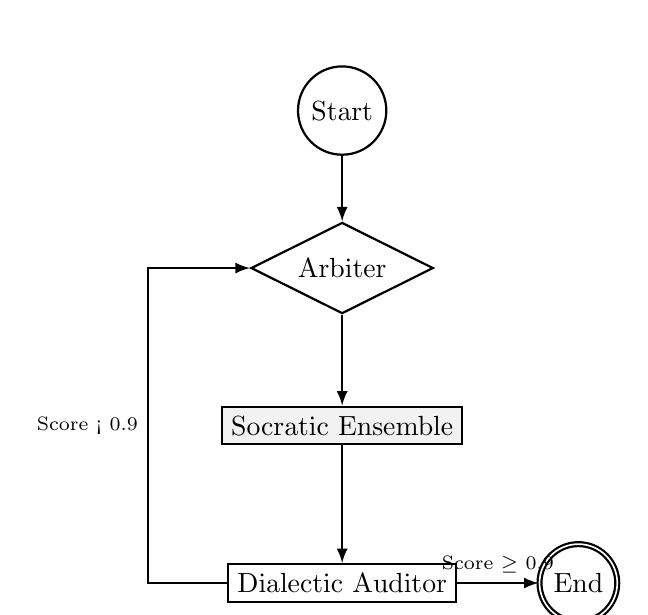
\begin{tikzpicture}[node distance=2cm, >=latex, thick]
        \node (start) [circle, draw] {Start};
        \node (arbiter) [diamond, draw, aspect=2, below of=start] {Arbiter};
        \node (agents) [rectangle, draw, below of=arbiter, xshift=0cm, fill=gray!10] {Socratic Ensemble};
        \node (dialectic) [rectangle, draw, below of=agents] {Dialectic Auditor};
        \node (end) [circle, double, draw, right of=dialectic, node distance=3cm] {End};
        
        \draw [->] (start) -- (arbiter);
        \draw [->] (arbiter) -- (agents);
        \draw [->] (agents) -- (dialectic);
        
        % The loop back logic
        \draw [->] (dialectic.west) -- ++(-1,0) |- (arbiter.west) 
            node [near start, left, font=\scriptsize] {Score < 0.9};
            
        % The exit logic
        \draw [->] (dialectic) -- (end) 
            node [midway, above, font=\scriptsize] {Score $\ge$ 0.9};
    \end{tikzpicture}
    
    \caption{SocraticGraph State Transition Diagram}
    \label{fig:socratic_flow}
\end{figure}

While Figure \ref{fig:socratic_flow} shows the general structure of the graph where \textit{Arbiter} has to pick another model, the way in which it does is one of the most unique parts of this multi-agentic framework. Instead of simply having one "teacher" agent, there are three agents specialized to cover different parts of the Socratic method.

\subsubsection{System Prompts}
The system prompts for each model were crafted around having an identity and a specific goal in the process of the Socratic method (hence their designations). While a simple prompt could have been chosen such as "question the user" for a single agent with the purpose of questioning, the diversity of each system prompt allows for specific, unique approaches that are tailored to the Socratic method.

\subsubsection{Model Choice}
Other than having tailored prompts, having multiple agents gives the opportunity for picking specialized Large Language Models (LLM) for each purpose. When running the command line interface with \texttt{context\_switch} set to \texttt{False}, all models run on Llama 3.1 with 8 billion parameters with \texttt{q2\_K} quantization. While this is sufficient for a usable experience, context switching on purely logical-based agents like \textit{Arbiter} or \textit{Dialectic} to a Large Language Model like Phi-4 Mini with 3.8 billion parameters and \texttt{q4\_K\_M} quantization is better because of the saved memory footprint, high inference speed and strong reasoning. Like \textit{Arbiter} and \textit{Dialectic}, \textit{Elenchus} also benefits from context switching; Mistral is great at following instructions and its \texttt{q3\_K\_S} quantization still allows for deep understanding and the "cross-examination" that \textit{Elenchus} is tasked with doing.
\begin{table}[H]
    \centering
    \caption{Agent Model Choice and Quantization Strategy}
    \label{tab:model_ensemble}
    \begin{tabular}{@{}llll@{}}
        \toprule
        \textbf{Node Role} & \textbf{Model Architecture} & \textbf{Quantization} & \textbf{Engineering Justification} \\ \midrule
            Arbiter   & Phi-4 Mini (3.8B)  & \texttt{q4\_K\_M} & High reliability for deterministic routing. \\
            Elenchus  & Mistral (7B)       & \texttt{q3\_K\_S} & Balanced for instruction following/debate. \\
            Aporia    & Llama 3.1 (8B)     & \texttt{q2\_K}    & Optimized for creative breadth over logic. \\
            Maieutics & Llama 3.1 (8B)     & \texttt{q2\_K}    & Leverages high parameter count for analogies. \\
            Dialectic & Phi-4 Mini (3.8B)  & \texttt{q4\_K\_M} & Strong reasoning for objective grading. \\ \bottomrule
    \end{tabular}
\end{table}

\subsection{Quantitative Mastery Evaluation}
To bridge the gap between qualitative LLM dialogue and deterministic program flow, SocraticGraph implements a regex-based extraction layer within the \texttt{Dialectic} node. The auditor is prompted to wrap its evaluation in a specific token: \texttt{[[SCORE: X.X]]}. 

The system utilizes Python's \texttt{re} module to parse this float, which then dictates the conditional edge traversal within the StateGraph class. This approach transforms subjective learning progress into a quantifiable metric, ensuring that the transition to the \texttt{END} state is strictly governed by a verified mastery threshold.

\subsection{Hardware Optimizations}
Closed source and high parameter, cutting edge models are meant to be run on expensive hardware and for a project targeting students, there is no reasonable expectation to have a thousand dollar Graphics Processing Unit for Large Language Models. The optimizations in the quantization and parameter sizes of the model (mentioned in Table \ref{tab:model_ensemble}) is a strong start for optimization, but the functions contained in \texttt{history.py} help to optimize for consumer hardware outside of the Ollama backend. Predefined in \texttt{history.py} but editable through the command line interface, a \texttt{context\_token\_budget} variable is defined. This variable bounds the total budget for context tokens and when the context tokens start to grow beyond the budget, they are removed in a \textbf{first-in-first-out (FIFO)} manner. While this number can be changed, the default 4096 value is enough to capture most of the history while staying within the constraints of 8GB VRAM on modern consumer hardware. 

\section{Conclusion}
SocraticGraph demonstrates the viability of executing complex, multi-agent pedagogical workflows on consumer-grade hardware. By implementing a directed acyclic graph (DAG) and multiple models with specialized tasks, the framework successfully mitigates the "direct-answer bias" inherent in monolithic LLM architectures. 

The integration of a deterministic evaluation layer ensures that instructional progress is measured quantitatively, while the use of local inference via Ollama preserves user data sovereignty. As AI continues to shift toward edge-computing, architectures like SocraticGraph provide a blueprint for private, specialized, and hardware-efficient learning tools. 

%Future work will involve expanding the \texttt{SocraticState} to include long-term memory via Vector Databases (RAG) to further personalize the learning journey.
\begin{thebibliography}{9}
\bibitem{langchain}
LangChain (2023). \textit{LangChain}. LangChain Inc. \url{https://github.com/langchain-ai/langchain}

\bibitem{langgraph}
LangChain (2024). \textit{LangGraph}. LangChain Inc. \url{https://github.com/langchain-ai/langgraph}

\bibitem{llama3}
Meta AI. (2024). \textit{The Llama 3 Herd of Models}. arXiv preprint arXiv:2407.21783.

\bibitem{phi4}
Microsoft Research. (2024). \textit{Phi-4 Technical Report}. 

\bibitem{mistral}
Mistral AI Research Team. (2023). \textit{Mistral 7B}. arXiv preprint arXiv:2310.06825.

\bibitem{ollama}
Ollama Team. (2023). \textit{Ollama}. \url{https://ollama.com}

\end{thebibliography}
%%% End document
\end{document}